% ============================================================================
% PAQ-KV — AAAI-27 submission draft, distilled from paq_living.tex (2026-07-17).
% Every number is taken verbatim from the living document; nothing re-derived.
% 2026-07-22 style revision (v2): prose reworked to match AB's register
% (no em dashes, no "beat" vocabulary, plain section titles); all numbers,
% tables, labels and citations unchanged.
% 2026-07-24: PAQ acronym defined (Prefill once, Ask many Queries); page-level
% labelling clarified; duplicate Figure 2 include removed (long caption kept);
% \ref{sec:limitations} retargeted to app:repro after that section was
% commented out (collaborator pass).
% Build: ./tectonic -X compile paq_aaai.tex
% ============================================================================
\documentclass[letterpaper]{article} % DO NOT CHANGE THIS
% ---------------------------------------------------------------------------
% LOCAL BUILD SHIM (this block only; the style file itself is untouched):
% the host has no pdflatex, so this draft is built with tectonic (XeTeX-based).
% aaai2027.sty's engine guard (\RequirePDFTeX) is neutralized ONLY when the
% engine is not pdfTeX. Under the official pdflatex build this block is inert
% and the guard runs as shipped. Remove the shim for the actual submission.
\usepackage{iftex}
\ifPDFTeX\else\let\RequirePDFTeX\relax\fi
% ---------------------------------------------------------------------------
\usepackage[submission]{aaai2027}  % DO NOT CHANGE THIS
\usepackage[hyphens]{url}  % DO NOT CHANGE THIS
\usepackage{graphicx} % DO NOT CHANGE THIS
\urlstyle{rm} % DO NOT CHANGE THIS
\def\UrlFont{\rm}  % DO NOT CHANGE THIS
\usepackage{natbib}  % DO NOT CHANGE THIS AND DO NOT ADD ANY OPTIONS TO IT
\usepackage{caption} % DO NOT CHANGE THIS AND DO NOT ADD ANY OPTIONS TO IT
\frenchspacing  % DO NOT CHANGE THIS
\usepackage{algorithm}
\usepackage{algorithmic}
\usepackage{booktabs}
\usepackage{multirow}
\usepackage{amsmath}
\usepackage{amssymb}


\pdfinfo{
/TemplateVersion (2027.1)
}

\setcounter{secnumdepth}{2}

\graphicspath{{figures/}}

\newcommand{\paq}{\textsc{PAQ}}
\newcommand{\paqt}{\textsc{PAQ-T}}
\newcommand{\paqc}{\textsc{PAQ-KV}}
\newcommand{\lb}{\mathrm{LB}_{95}}

\newcommand{\jiahui}[1]{\textcolor{red}{[Jiahui: #1]}}

\title{Prefill Once, Ask Many: Training-Free Reversible Below-Page KV Selection\\for Multi-Query Long-Document Visual Question Answering}
\author{
    Anonymous submission
}
\affiliations{
    Anonymous submission
}

\begin{document}

\maketitle

\begin{abstract}
Long-context vision-language models can answer questions about multi-page documents, but repeatedly reading the full document is costly. Existing KV-cache eviction methods address this by committing to one compressed context, even when later questions require different evidence. We present \paqc{} (``Prefill once, Ask many Queries''), a training-free architecture for reversible, query-specific context selection in multi-query document visual question answering. \paqc{} prefills a document once and retains its complete KV cache. For each question, it uses the frozen reader's own question-to-content attention to score 64-token page-aligned blocks, then restricts decoding to the selected blocks with a four-dimensional additive attention mask. The retained document cache is neither gathered nor discarded, allowing every question to select a different view without an additional model, retrieval index, or document re-read. Per-query selection outperforms committing the same scorer once, by $0.264$ in a clean-cache comparison and $0.379$ in a block-level replication. At a nominal 5\% decode-attention budget (${\approx}6\%$ realized), \paqc{} scores $0.4042$ on MMLongBench-Doc versus $0.3282$ for the trained ColQwen2 retriever, while remaining statistically indistinguishable from full-context decoding and the gold-page oracle on the development pin. A single evaluation on a fresh, disjoint, sealed 45-document/244-query set confirms the \paqc{}--ColQwen2 improvement ($0.396$ versus $0.320$; $+0.076$, document-clustered $\lb=+0.029$). On LongDocURL, \paqc{} matches but does not outperform ColQwen2 and remains slightly below full-context decoding. Retaining the complete cache while selecting a new context for each question is therefore an effective alternative to irreversible eviction for multi-query document understanding.
\end{abstract}

\section{Introduction}\label{sec:intro}

% Figure source: BASED/research/paq_sealed_final_sealed_verdict.json
\begin{figure}[t]
\centering
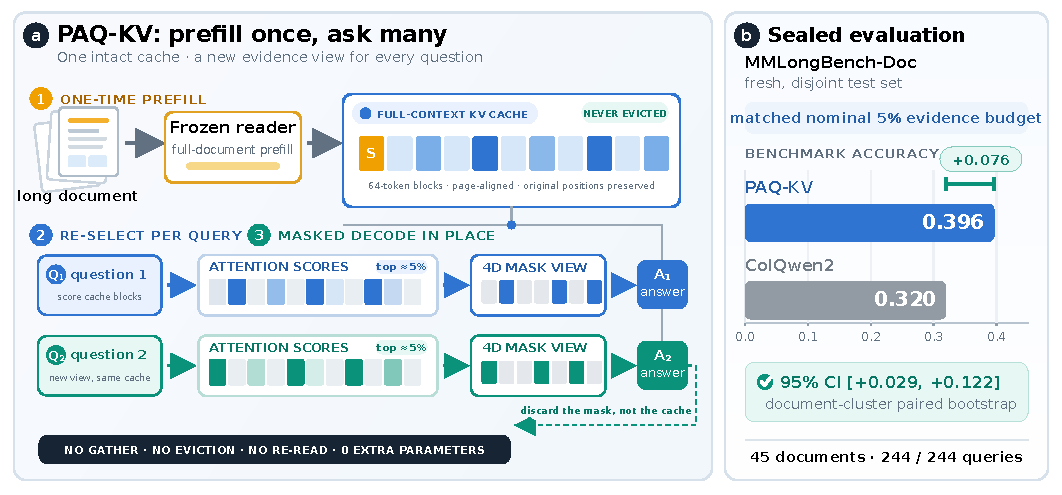
\includegraphics[width=\columnwidth]{figures/figure1_paq_kv_no_overlap_v3.pdf}
\caption{Method and sealed result at a glance. On fresh, disjoint MMLongBench-Doc, \paqc{}@5\% scores $0.396$ versus $0.320$ for corrected-loader ColQwen2 ($+0.076$, document-clustered 95\% CI $[+0.029,+0.122]$; 45 documents, 244/244 queries).\jiahui{this figure is too close to Figure 2, need to change}}
\label{fig:overview}
\end{figure}

Long-context vision-language models (VLMs) can read an entire multi-page document, but they pay for every page on every question. The standard efficiency response, inherited from single-query text benchmarks, is to \emph{evict}: keep a compact subset of the KV cache and decode against it \citep{li2024snapkv,zhang2023h2o,chen2024fastv,wan2024lookm,kim2025kvzip}. Eviction is a single, irreversible commitment: whatever subset is kept must serve every future question about that document.

In practice, however, document assistants are not asked one question. The two long-document VQA benchmarks we use are natively multi-query: grouping their 64K splits by source document, MMLongBench-Doc \citep{ma2024mmlongbench} averages ${\approx}6.97$ questions per document and LongDocURL \citep{deng2025longdocurl} ${\approx}3.6$; inside our pinned evaluation subsets the averages are 5.50 and 5.79 gold-bearing questions per document. Different questions need different evidence, so a subset committed for question~1 is stale for question~5.

This paper asks whether, at a matched budget on long multimodal documents, per-query \emph{re-selection} of context outperforms a \emph{commit-once} selection, and whether a training-free, reader-internal selector can compete with a dedicated trained retriever. Our answer is \paqc{} (Prefill once, Ask many Queries): prefill the full document once into the KV cache of a frozen reader (Qwen3-VL-8B; \citealp{qwen3vl2025}) and retain it; per query, re-select the most relevant 64-token, below-page KV blocks with the reader's own question$\to$content attention; decode under a restricted-attention 4D mask over the retained full-context cache. Nothing is discarded and nothing is gathered (M-RoPE positions are untouched), so a selection is a view of the cache rather than a commitment: the next question re-selects from the same intact cache. Figure~\ref{fig:overview} summarizes the architecture and its sealed MMLongBench-Doc result.

\paragraph{Contributions.}
\begin{itemize}
\item \textbf{A reversible below-page architecture and its tested mechanism.} \paqc{} keeps the full-document prefill intact and, per query, re-selects 64-token below-page KV blocks and decodes under a 4D restricted-attention mask without gathering the cache, so all M-RoPE positions stay the model's own. Under a pre-registered two-comparator gate, per-query re-selection outperforms the identical scorer committed once ($+0.257$/$+0.163$ per cell; 903 queries, 80 documents/cell, document-clustered) and a strong gold-informed static ($+0.108$/$+0.104$); the contrast survives a clean-cache re-run ($+0.264$, $\lb=+0.187$), reappears below page level ($+0.379$, $\lb=+0.273$), and also holds for a trained retriever's committed form.
\item \textbf{An out-of-sample-confirmed improvement, with explicit bounds and negative results.} On MMLongBench-Doc, \paqc{} at a nominal 5\% (realized ${\approx}6\%$) budget scores $0.4042$ vs.\ ColQwen2 $0.3282$ ($+0.077$, $\lb=+0.040$; 80 documents, 444 decoded / 440 paired; ColQwen2 evaluated with its trained retrieval-projection LoRA correctly loaded, \S\ref{sec:integrity}), is indistinguishable from full context, and is not statistically distinguishable from the gold-page oracle at its ${\sim}6\%$ budget ($-0.026$, with a confidence interval that straddles zero); the improvement also holds on a fresh, disjoint, sealed set ($+0.076$, $\lb=+0.029$). On LongDocURL \paqc{} matches but does not outperform ColQwen2 ($+0.019$, $\lb=-0.019$; below full context by $-0.014$), and both the per-head mixture transfer gate and the sharp expert-head scorer failed their pre-registered gates.
\end{itemize}

\paragraph{Evidence status.} Primary full-method accuracy results use the 80-document-per-cell development pins unless explicitly labelled otherwise; the mechanism, budget, and integrity analyses use the stated subsets (30/24/50-document and 157-query screens). Only the MMLongBench-Doc \paqc{}-versus-ColQwen2 comparison was evaluated on the sealed set: once, on a fresh, disjoint 45-document / 244-query cell, where the improvement holds ($+0.076$, $\lb=+0.029$; \S\ref{sec:results-mmlo}). The sealed LongDocURL documents remain unevaluated (out of scope for this MMLongBench-scoped result). We state the evidence status wherever it matters.

\section{Related Work}\label{sec:related}

\paragraph{Page selection and retrieval.} CAPS \citep{zhu2026caps} publishes attention-based \emph{page} selection on our benchmarks, and ColPali/ColQwen2 \citep{faysse2025colpali} are the strongest trained retrieval baselines we compare against. We are explicit that selecting pages with reader attention is CAPS's method; \paqc{} differs on the axes CAPS names as open: below-page granularity, reversible per-query re-selection over one retained prefill in the multi-query regime, and direct masked decode from the retained cache with no re-read.

\paragraph{KV-cache eviction.} SnapKV \citep{li2024snapkv}, H2O \citep{zhang2023h2o}, FastV \citep{chen2024fastv}, LOOK-M \citep{wan2024lookm}, and KVzip \citep{kim2025kvzip} commit a compressed cache once; Quest \citep{tang2024quest} shows that query-aware selection can outperform query-agnostic eviction in single-query text, which motivates but does not prove our multi-query claims. Our search did not identify prior work in the exact combined setting of reader-internal attention as the runtime below-page selector, end-to-end QA at matched budget against page-level retrieval, and long multi-query documents; we offer this as a provisional reading of the literature, not as proof of novelty.

\section{Method: \paqc{}}\label{sec:method}

\subsection{Setting}
One long visual document, consumed as page images (no OCR), is read by a frozen VLM and will be asked $k$ questions (5.5 to 5.8 gold-bearing per document in our pins). The document is prefilled \emph{once} at the same rendering the full-context arm uses (a nominal ${\approx}64$K-token target; realized prefill lengths reach ${\approx}92$K on the largest pinned documents) and the KV cache is retained: never evicted, never physically compressed, never gathered. The cache plays the role that a multi-vector index plays for a retriever, except that it is the reader's own working memory, so retrieval and reading share one representation and one model.

\subsection{Per Query: Preview, Re-Select, Masked Decode}
\begin{enumerate}
\item \textbf{Preview (score).} The tokenized question is forwarded over the retained cache (crop-restored afterwards so queries never contaminate one another; \S\ref{sec:integrity}), and the question rows' attention over context positions is aggregated into scores over 64-token, page-aligned KV blocks: fine enough to isolate a table row, a figure caption, or a paragraph, while remaining coarse enough for the scores to be stable.
\item \textbf{Re-select.} Keep the top-scoring blocks at a nominal 5\% decode-attention budget. We use this terminology deliberately: the kept blocks' K/V were computed with full-document context during the prefill (the standard claim semantics of the Quest/SnapKV method class), so this is a decode-attention budget rather than a matched-token prefill comparison; the realized attended fraction on the executed screen is ${\approx}5.9$ to $6.0\%$ of context and is always reported. The matched quantity against ColQwen2 is the evidence budget (5\% of pages vs.\ 5\% of context) at the same shared reader and QA evaluator; the two methods' \emph{selection} scorers differ (reader attention vs.\ the trained ColQwen2 retriever).
\item \textbf{Masked decode.} The answer is generated while attending only to the selected blocks plus a small always-keep set (the BOS/system/template scaffold, the question itself, and previously generated tokens), enforced by a 4D additive attention mask (batch, head, query row, key) over the retained cache. There is no gathering: the K/V tensors stay at their original positions, so every M-RoPE rotary index is exactly the model's own, and the failure mode that makes physical cache-gathering error-prone for VLMs does not arise. There is no re-read, no re-render, no second model.
\end{enumerate}

\paragraph{Formal definition.}
Let $Q_j$ be the token positions of question $j$, let $V$ be the visual-content positions, and let $B_1,\ldots,B_m$ be the page-aligned blocks partitioning $V$. For attention probability $A_{\ell h}(r,t)$ from question row $r$ to context position $t$ at layer $\ell$ and head $h$, the default scorer averages over all $L$ layers, $H$ heads, and question rows, then averages within each block:
\begin{equation}
\begin{aligned}
\alpha_j(t)&=\frac{1}{LH|Q_j|}\sum_{\ell=1}^{L}\sum_{h=1}^{H}
                  \sum_{r\in Q_j}A_{\ell h}(r,t),\\
s_j(B_i)&=\frac{1}{|B_i|}\sum_{t\in B_i}\alpha_j(t).
\end{aligned}
\label{eq:block-score}
\end{equation}
Let $\pi_j$ order blocks by decreasing $s_j$. At budget $b$, selection stops at the first block whose inclusion reaches the visual-token budget:
\begin{equation}
\begin{aligned}
r_j&=\min\left\{r:\sum_{u=1}^{r}|B_{\pi_j(u)}|\geq b|V|\right\},\\
S_j&=\bigcup_{u=1}^{r_j}B_{\pi_j(u)}.
\end{aligned}
\label{eq:block-select}
\end{equation}
If $A$ denotes the always-keep scaffold and $G_j$ the generated-token positions, define $T_j(x)=A\cup S_j\cup\{t\in Q_j\cup G_j:t\leq x\}$. The additive mask for decode row $x$ is
\begin{equation}
M_j(x,t)=
\begin{cases}
0, & t\in T_j(x),\\
-\infty, & \text{otherwise}.
\end{cases}
\label{eq:restricted-mask}
\end{equation}
This row-wise mask is broadcast over batch and heads. After preview and decoding, the cache is cropped back to the document boundary, so the same retained document cache is used to construct $S_{j+1}$.

Algorithm~\ref{alg:paqc} (Appendix~\ref{app:method-materials}) gives the loop and Figure~\ref{fig:paqkvmask} shows the mask machinery. Attention is captured by per-layer forward hooks that reduce each layer's attention tensor immediately and discard it, so peak memory is one layer's attention (the naive all-layers path runs out of memory at long contexts).

% Figure validation source: BASED/research/paqc_identity_audit.json (zero mask-specific argmax changes)
\begin{figure*}[t]
\centering
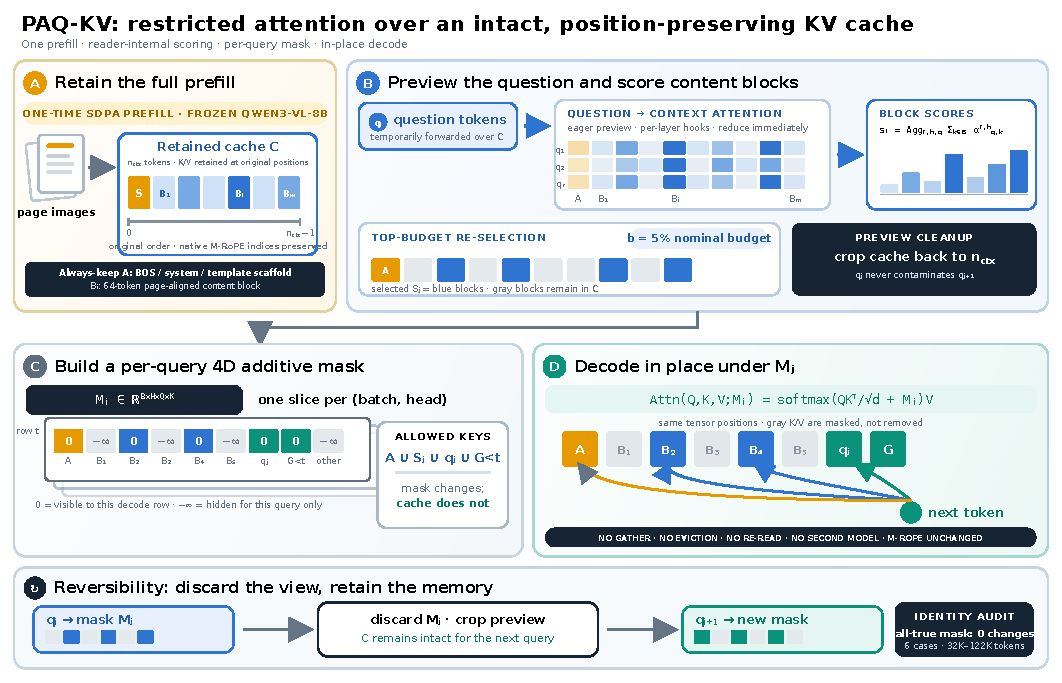
\includegraphics[width=0.92\textwidth]{figures/figure2_paq_kv_detailed_v1.pdf}
\caption{
Detailed PAQ-KV restricted-attention mechanism.
\textbf{A:} The frozen reader prefills the document once and retains the full KV cache \(C\), including the always-keep scaffold \(A\) and page-aligned 64-token blocks \(B_1,\ldots,B_m\), at their native M-RoPE positions.
\textbf{B:} For each question \(q_j\), an eager-attention preview captures question-to-context attention using per-layer hooks. Attention mass is aggregated into block scores, and the highest-scoring blocks \(S_j\) are retained under the nominal \(5\%\) decode-attention budget. The preview is then cropped so that questions cannot contaminate subsequent queries.
\textbf{C:} PAQ-KV constructs a query-specific additive mask \(M_j \in \mathbb{R}^{B \times H \times Q \times K}\), assigning \(0\) to \(A \cup S_j \cup q_j \cup G_{<t}\) and \(-\infty\) to all other keys.
\textbf{D:} Decoding proceeds directly over the intact cache under \(M_j\), without gathering or evicting K/V, re-reading the document, or changing positional indices. After answering, \(M_j\) is discarded, and the same complete cache is re-masked for \(q_{j+1}\).
}\label{fig:paqkvmask}
\end{figure*}

\subsection{Exactness and Reversibility}
A decode-identity audit checked the mask path against the native decode over 6 document-query pairs deliberately spanning $32$K to $122$K tokens (a stress range wider than the ${\le}64$K evaluation pin, chosen to probe long-context behavior): in all 6 audited cases an all-true mask produced zero mask-specific argmax changes relative to the native causal decode (an earlier single greedy-token divergence traced to the generation loop's mask-independent fast-path kernel, not to the mask). We therefore claim that the mask decode is identical to the native decode in the audited cases, not that this holds in general; this audit was a pre-registered kill criterion. Because nothing is discarded, a selection is a view rather than a commitment: the next query re-scores and re-masks the same complete cache, whereas commit-once eviction cannot, since whatever it dropped is unrecoverable. Reversibility is our tested axis (\S\ref{sec:setup-stats}), and the contrast replicates at block level ($+0.379$, $\lb=+0.273$; \S\ref{sec:results-mmlo}).

\paragraph{Relation to existing designs.} \paqc{} is not CAPS (a separate scoring VLM, per-page full re-forwards, page granularity, single-query); it is not coarse-to-fine page routing with a full-resolution re-read (\paq{}~v1, our own earlier page-level system, Appendix~\ref{app:pagelevel}); and it is not eviction (the mask is per-query and reversible). The mask route is the \emph{accuracy} path; physically gathering the cache for savings is a separate efficiency claim, and one we do not make here.

\section{Experimental Setup}\label{sec:setup}

\subsection{Benchmarks, Pins, Reader}
We evaluate on LongDocURL \citep{deng2025longdocurl} and MMLongBench-Doc \citep{ma2024mmlongbench}, both as page images. For each document we build the union of the benchmark's own-document pages across that document's queries (dropping cross-document 64K padding), so every query's evidence is present in one prefill. Documents qualify with $\geq 3$ gold-bearing queries and $\leq 110$ union pages (a nominal ${\approx}64$K-token target at read resolution; realized lengths reach ${\approx}92$K on the largest documents); selection is seed-0 frozen. The confirmatory pin holds 80 documents per cell with 463/440 complete queries and 5.79/5.50 gold-bearing queries per document (LongDocURL/MMLongBench-Doc; Appendix~\ref{app:method-materials}); a 30-document screen pin is its strict prefix, and results are additionally checked on the 50 new documents only (\S\ref{sec:results-isolation}). The reader is Qwen3-VL-8B \citep{qwen3vl2025}, frozen (scaled dot-product attention (SDPA) for prefill and reading; eager attention only during the per-query attention preview, so that question$\to$content scores can be captured). Page-level arms operate at a matched page budget $b \in \{2.5\%, 5\%, 10\%\}$ (the pre-registered gate budget is $b=5\%$); accuracy is the benchmark's document-VQA scorer. Everything in this paper is a Qwen3-VL-8B case study; no second reader VLM has been evaluated.

\subsection{Statistical Protocol}\label{sec:setup-stats}
All inference uses a document-cluster paired bootstrap: queries of one document share the document and (for stale arms) the single committed subset, so bootstrapping over queries would be anti-conservative pseudoreplication. Intervals resample documents with replacement within each cell (10{,}000 draws, seed 0); $\lb$ denotes the 2.5th percentile of the bootstrap distribution, that is, the lower end of a two-sided 95\% CI. Per-cell results are primary; pooled contrasts use equal cell weighting and are labelled. Every gate in this study was frozen before its run.

\paragraph{The isolation gate.} That query-aware selection outperforms query-agnostic eviction is both a known text result \citep{tang2024quest} and a potential strawman. We therefore fix the tested axis to \emph{reversibility}: every baseline runs its canonical scorer but is deployed stale, committed once per document (query-aware scorers commit a min-max-normalized aggregate over the document's first $M=\min(3,k)$ queries), while the fresh arm re-selects per query. Reversibility is credited only if the fresh arm outperforms both (i) its \emph{own} scorer committed once (identical scorer and budget, so the delta isolates the mechanism) and (ii) a strong \emph{gold-informed} static subset (top pages by gold-page frequency across the document's queries; not deployable, and not provably optimal, but immune to the weak-static artifact that invalidated an earlier one-comparator gate).

\subsection{Baselines}
The executed panel (Appendix~\ref{app:panel}) compares, per query at matched budget on the same pinned data and reader: ColQwen2 \citep{faysse2025colpali} fresh and stale, CLIP \citep{radford2021clip} fresh, SnapKV fresh/stale, the isolation arms above, random/truncation controls, and a query-blind eviction family (H2O; a context-only FastV proxy; LOOK-M; a KVzip \texttt{recv\_max} proxy). The eviction arms are disclosed proxies that sit at or below random page recall on these cells, and we rest no claim on outperforming them. Full-context and gold-page-oracle rows are references, not competitors.

\subsection{Methods Integrity}\label{sec:integrity}
An independent code review found a real bug in the per-query scoring loop used across this study: the runtime mutates the retained cache in place, and the loop reused the document prefill across a document's queries without restoring it, so query $q_i$ scored while attending to $q_0\ldots q_{i-1}$. The fix (crop the cache after every per-query preview) is now applied everywhere, and its impact was quantified rather than assumed: on a 24-document/150-query clean-vs-polluted re-run, the key isolation contrast is $+0.264$ ($\lb=+0.187$) clean vs.\ $+0.284$ polluted, since the contrast largely cancels the bug when both arms share the same scorer; absolute fresh-arm accuracy, in contrast, carries ${\approx}0.04$ inflation in the (page-level, pre-fix) confirmatory run, which we disclose wherever absolute levels matter. All \paqc{} results postdate the fix.

\paragraph{Baseline-loader integrity.} A second independent review caught a defect in the \emph{comparator}, not in our method: the cached ColQwen2 baseline had run with its trained final retrieval-projection LoRA (\texttt{custom\_text\_proj}) silently zeroed. \texttt{vidore/colqwen2-v1.0} is a PEFT adapter, and under our peft/transformers versions a key remap inserted \texttt{language\_model} into the LoRA target path (correct for the language-model layers but wrong for the top-level \texttt{custom\_text\_proj}), so the checkpoint's projection-LoRA tensors landed at a non-matching path and the final projection ran with a zero LoRA delta (base weights only). Because the other adapter layers still loaded, the baseline was functional (well above random), which masked the defect until we inspected the load report and the projection weights directly. We patched the loader (the two checkpoint \texttt{custom\_text\_proj} LoRA tensors are copied onto the correct module, and a post-load assertion now verifies they match the checkpoint) and re-scored ColQwen2 with the corrected loader. The correction is immaterial to the main result: fixed-vs-broken gold-page recall@5\% is $0.539$ vs.\ $0.534$ ($+0.005$), the top-5\% page selections overlap at Jaccard $0.947$ (only $34/444$ queries change any selected page), and re-reading those changed queries moves fresh-read accuracy by $-0.0002$ ($0.3282$ corrected vs.\ $0.3284$ broken); the improvement is $+0.077$ ($\lb=+0.040$) against the corrected ColQwen2 and $+0.077$ ($\lb=+0.039$) against the broken one. The trained projection LoRA does not materially reorder ColQwen2's rankings on this MMLongBench-Doc data, so the main result is not loader-inflated. The corrected loader is used for the main MMLongBench-Doc comparison (development and sealed) and the systems measurement; the LongDocURL result and the historical page-level panel retain the earlier (uncorrected) loader and are labelled as such. We do not infer a direction for the correction on the cells that were not re-run: on MMLongBench-Doc the change was negligible in both directions (gold-recall $+0.005$; fresh-read QA $-0.0002$), and LongDocURL, already a matched result rather than an improvement, is reported as an uncorrected-loader development result.

Separately, this study adopted a sealed-test discipline: the 80-document pin is development-only, and a fresh, disjoint 45-document / 244-query MMLongBench-Doc set (zero overlap with the pin) was reserved and evaluated \emph{exactly once} under a frozen harness. The confirmatory bar, comparator, budget, imputation policy, and all eight component code hashes were frozen (and a byte-hash of the sealed pin recorded) before the single run, and a guard enforces this. That one sealed evaluation confirms the improvement out-of-sample (\S\ref{sec:results-mmlo}); the sealed LongDocURL documents were not evaluated (out of scope for this MMLongBench-scoped result).

\section{Results}\label{sec:results}

\subsection{Isolating Reversibility}\label{sec:results-isolation}

At $b=5\%$ on 903 complete queries (80 documents/cell), the fresh page-level selector (\paq{}, Appendix~\ref{app:pagelevel}) scores $0.386$/$0.258$ (LongDocURL/MMLongBench-Doc) vs.\ $0.128$/$0.095$ for the \emph{identical scorer committed once} and $0.278$/$0.154$ for the gold-informed static: fresh $-$ commit-once is $+0.257$/$+0.163$ and fresh $-$ static is $+0.108$/$+0.104$, and both cells pass the gate (full table in Appendix~\ref{app:method-materials}; Figure~\ref{fig:reversibility} shows the tested axis schematically with every executed isolation interval).
Three robustness checks follow. (i) \emph{Independent extension}: because the screen pin is embedded in the confirmatory pin, we re-ran the statistics on the 50 new documents per cell only ($n=582$ queries): fresh $-$ commit-once $+0.216$ $[+0.159,+0.269]$; fresh $-$ static $+0.108$ $[+0.059,+0.150]$. (ii) \emph{Clean-cache re-run}: the contrast survives the integrity fix of \S\ref{sec:integrity} ($+0.264$, $\lb=+0.187$). (iii) \emph{Scorer generality}: the same fresh-over-stale collapse holds for a retrieval scorer, with ColQwen2 fresh at $0.423$ vs.\ stale at $0.178$ (query-micro; equal-cell $0.420$ vs.\ $0.177$), so reversibility is a property of the multi-query regime rather than of our scorer. A pre-registered ``commitment-pressure'' mechanism gradient failed its formal interaction test (both intervals include zero) and is retained as exploratory only; we make no mechanism-gradient claim.

\subsection{MMLongBench-Doc Results}\label{sec:results-mmlo}

\begin{table*}[t]
\centering\small
\begin{tabular}{lcc}
\toprule
 & LongDocURL & MMLongBench-Doc \\
\midrule
\paqc{}@5\% (ours) & \textbf{0.5315} & \textbf{0.4042} \\
ColQwen2-fresh (matched budget) & 0.5124 & 0.3282 \\
full-context (reference) & 0.5456 & 0.3965 \\
gold-page oracle (reference; not strict) & 0.6092 & 0.4314 \\
\midrule
\paqc{} $-$ ColQwen2-fresh & $+0.019$ $[-0.019,+0.059]$ & $+0.077$ $[+0.040,+0.115]$ \\
\paqc{} $-$ full-context & $-0.014$ (n.s.) & $+0.009$ $[-0.022,+0.040]$ \\
\paqc{} $-$ gold-page oracle & n/a & $-0.026$ $[-0.059,+0.008]$ \\
\midrule
Queries (decoded / paired) & 463 / 463 & 444 / 440 \\
Pre-frozen bar (per-cell $\lb>0$) & \textsc{not met} & \textbf{\textsc{met}} \\
\bottomrule
\end{tabular}
\caption{\paqc{} at the 80-document development pin, nominal 5\% budget (all values on the same 80-document development cohort; document-cluster paired bootstrap; contrast rows report $\Delta\,[\lb,\mathrm{UB}_{95}]$). All four accuracy rows are the verified 80-document development-pin means; no 30-document screen values are mixed in. On LongDocURL \paqc{} is \emph{below} full-context ($-0.014$, not significant); on MMLongBench-Doc it is indistinguishable from full-context. MMLongBench-Doc decodes 444 queries; the paired contrasts against the cached ColQwen2-fresh, full-context, and gold-oracle rows are computed on the 440 queries with cached references (the 4 \texttt{mi\_phone} rows lack cached references).}
\label{tab:paqkv}
\end{table*}

\paragraph{Main comparison.} On the 80-document development pin (444 queries decoded; contrasts on the 440 with cached references), \paqc{}@5\% scores $0.4042$ vs.\ ColQwen2-fresh $0.3282$: $+0.077$ with $\lb=+0.040$, which meets the pre-frozen per-cell bar with margin (Table~\ref{tab:paqkv}). ColQwen2 here is loaded with its trained retrieval-projection LoRA correctly applied; \S\ref{sec:integrity} documents a loader defect we found and corrected, and shows that the correction is immaterial to this comparison.

\paragraph{Out-of-sample confirmation.} The improvement holds on a fresh, disjoint, sealed set evaluated exactly once. On 45 MMLongBench-Doc documents / 244 queries with zero overlap with the development pin, under a frozen harness whose bar, comparator, budget, imputation policy, and code hashes were all pre-registered (\S\ref{sec:integrity}), \paqc{}@5\% scores $0.396$ vs.\ ColQwen2-fresh $0.320$: $+0.076$, document-clustered $\lb=+0.029$, complete ($244/244$, zero skips) and unchanged under worst-case missingness imputation. The pre-registered verdict (complete-case $\lb>0$, with an adversarial-imputation fallback that binds only if any query is missing) is met. The sealed effect ($+0.076$) closely matches the development-pin estimate ($+0.077$); the sealed interval is appropriately wider ($\lb=+0.029$ vs.\ $+0.040$) at the smaller held-out sample. Only the \paqc{}-vs-ColQwen2 comparison was sealed-evaluated; the full-context and gold-page-oracle reference arms above are development-pin only and were not run on the sealed set. This single out-of-sample evaluation is the strongest evidence in the paper and directly addresses the reuse of the development pin across this study (disclosed in Appendix~\ref{app:repro}). \paqc{} attends to a nominal 5\% (realized ${\approx}5.9$ to $6.0\%$) of the context; at that budget it is indistinguishable from full context ($+0.009$ $[-0.022,+0.040]$) and not statistically distinguishable from the gold-page oracle ($-0.026$ $[-0.059,+0.008]$). The latter interval permits material inferiority, so this is parity within noise rather than demonstrated equality.

\paragraph{Mechanism checks.} On the 30-document screen (distinct from the 80-document cohort above), the result survives every mechanistic adversarial check: it is query-dependent (\paqc{} $-$ random-block selection $= +0.329$ $[+0.238,+0.418]$), query-specific (\paqc{} $-$ wrong-question selection $= +0.698$ $[+0.603,+0.784]$, where the collapse supports query-specificity), reversible (\paqc{} $-$ commit-once $= +0.379$ $[+0.273,+0.480]$), and below-page granularity helps over page level ($+0.054$ $[+0.011,+0.102]$). These are development-pin screen analyses with disclosed caveats: the screen budget-curve monotonicity gate failed on this cell ($0.398$ at 10\% vs.\ $0.402$ at 5\%), and the effect they dissect is separately confirmed out-of-sample on the sealed set above.

\paragraph{Additional matched-budget baselines.} On the same 80-document pin and reader, a BM25 page retriever scores $0.2109$ at matched 5\% budget and \paqc{} exceeds it by $+0.193$ ($\lb=+0.152$; 444 queries), while a training-free \emph{page-level} CAPS-style expert-head control scores $0.3561$ and below-page \paqc{} exceeds it by $+0.048$ ($\lb=+0.009$; 444 queries; unchanged under worst-case missingness imputation). The margin over this control is real but thin, so the improvement over the \emph{trained retriever} remains the stronger claim; the screen-only budget-sweep details are in Appendix~\ref{app:budget-sweep}.

\subsection{LongDocURL Results}\label{sec:results-longdocurl}

On the 80-document development pin (463 queries), \paqc{}@5\% scores $0.5315$ vs.\ ColQwen2-fresh $0.5124$: $+0.019$ with $\lb=-0.019$, a positive point estimate that does not meet the pre-frozen bar; on this cell \paqc{} also sits below full context ($-0.014$, not significant). The mechanism checks (query dependence, reversibility) pass here too; what is missing is the margin. We treat this as a bounding observation on where below-page selection helps rather than a second main result, and defer the conversion-bound decomposition to Appendix~\ref{app:limitations-detail}.

\subsection{Negative Results}\label{sec:results-negatives}

\paragraph{Per-head mixture transfer gate.} No LoRA adapter was ever trained: this pre-frozen check failed first and stopped that line of work. We fit a logistic per-head mixture over all $36{\times}32=1{,}152$ (layer, head) question$\to$page attention channels on off-benchmark provenance-checked data. The transfer gate fails: mixture gold-page recall is $0.652$/$0.594$ vs.\ $0.676$/$0.616$ for the single head, with pooled mixture $-$ single $=-0.023$ $[-0.037,-0.008]$ (907 queries), so the mixture overfits and this direction was closed. The best zero-benchmark-contact head (L21.H18) still coincides with the benchmark-supervised expert layer.

\paragraph{Sharp expert head as block scorer.} Replacing \paqc{}'s diffuse mean-attention block scorer (V0) with the sharp head L21.H18 (V1) fails the pre-frozen gate: on LongDocURL it only nudges the point estimate ($0.5315 \to 0.536$; V1 $-$ ColQwen2 $= +0.024$ $[-0.012,+0.066]$) and does not separate from V0 ($\lb(\mathrm{V1}-\mathrm{V0}) = -0.011$, n.s.), while on MMLongBench-Doc it hurts ($0.402 \to 0.381$ on the screen documents). As elsewhere in this study, recall-optimized selection is not accuracy-optimized selection.

\subsection{Systems Measurements}\label{sec:results-efficiency}
We measured the deployment profile of the true \paqc{} path (below-page masked decode over the \emph{retained} full-document KV cache) against ColQwen2-fresh and full context on an 8-document / 31-query systems subset of the pin (single RTX PRO 6000; frozen configuration; Table~\ref{tab:systems}); this corrects an earlier internal accounting that timed a different page-routing variant. Per online query, \paqc{} costs $1.04$\,s ($0.19$\,s selection $+$ $0.85$\,s masked decode), excluding ${\approx}1.99$\,s/query of removable research-harness input reconstruction (component sum ${\approx}3.03$\,s/query), versus ColQwen2's $0.46$\,s: \paqc{} is ${\approx}2.25\times$ \emph{slower} and far heavier in resident state (${\approx}8.15$\,GiB/document retained cache vs.\ ${\approx}11$\,MiB index, ${\approx}730\times$; peak VRAM $44.5$ vs $21.8$\,GiB), though it is ${\approx}11\times$ faster than full-context re-reading per query ($1.04$ vs $11.6$\,s; amortized crossover $N{\approx}1.07$ queries/document). The efficiency claim is therefore simplicity and deployment shape, not speed: no separately trained retriever checkpoint ($0$ extra trained parameters vs.\ $2.246$\,B), no stored vector index, one deployed model, and reversible query-time selection.

\begin{table}[t]
\centering\small
\setlength{\tabcolsep}{4pt}% permitted narrowing (AAAI kit)
\begin{tabular}{lcccc}
\toprule
 & extra & per-doc & online & peak \\
 & params & state & lat./q & VRAM \\
\midrule
\paqc{} (ours)   & $0$        & $8.15$\,GiB & $1.04$\,s  & $44.5$\,GiB \\
ColQwen2-fresh   & $2.246$\,B & $11$\,MiB   & $0.46$\,s  & $21.8$\,GiB \\
full-context     & $0$        & n/a         & $11.59$\,s & $44.6$\,GiB \\
\bottomrule
\end{tabular}
\caption{Deployment profile on an 8-document / 31-query systems subset (frozen configuration, single GPU). ``Extra params'' = additional retriever/selector parameters beyond the shared reader. \paqc{} is ${\approx}2.25\times$ slower and far heavier in resident state than ColQwen2, and ${\approx}11\times$ faster than full context (cold-start amortized after $N{\approx}1.07$ queries/document). \paqc{}'s online latency excludes ${\approx}1.99$\,s/query of removable research-harness input reconstruction (component sum ${\approx}3.03$\,s/query in the current implementation); mean generated lengths differ across arms ($5.3$/$3.5$/$4.1$ tokens for \paqc{}/ColQwen2/full-context). The advantage is $0$ extra retriever parameters, no index, one model, and reversible query-time selection, not speed.}
\label{tab:systems}
\end{table}

% \section{Limitations}\label{sec:limitations}
% \jiahui{Limitation section is not necessary in AAAI paper, we can remove.}
% \begin{itemize}
% \item \textbf{Reused development pin (adaptive-reuse caveat), with the main result confirmed out-of-sample.} Most \paqc{} numbers come from the 80-document development pin, which has been reused across this study's screening, auditing, and gating; pre-registered gates limit but do not eliminate the resulting adaptive-analysis/multiple-comparisons risk, so the development-pin \emph{analyses and ablations} remain development-grade. The main MMLongBench-Doc comparison is the exception: it is confirmed out-of-sample on the fresh, disjoint, sealed 45-document / 244-query set, evaluated exactly once ($+0.076$, $\lb=+0.029$; \S\ref{sec:results-mmlo}). That sealed cell (244 queries) sits just below the study's 250-query power floor, so its interval is appropriately wider than the development pin's; the sealed LongDocURL documents remain unevaluated (out of scope for this MMLongBench-scoped result).
% \item \textbf{One cell of two.} The improvement is confined to the dispersed-evidence regime; on LongDocURL the retriever is matched, not outperformed.
% \item \textbf{Single reader.} All results are a Qwen3-VL-8B case study; generalization to other VLMs is untested.
% \item \textbf{Budget semantics.} The \paqc{} budget is a nominal 5\% decode-attention budget (realized ${\approx}5.9$ to $6.0\%$) with block K/V computed under full-document prefill context: Quest/SnapKV claim semantics, not a matched-token prefill comparison.
% \item \textbf{No speed advantage (measured, not deferred).} \S\ref{sec:results-efficiency} measures the deployment profile on a systems subset: \paqc{} is ${\approx}2.25\times$ \emph{slower} per query and far heavier in resident state (${\approx}730\times$) than ColQwen2, and only ${\approx}11\times$ faster than full context. The efficiency argument is simplicity and deployment shape (no separately trained retriever, no index, one model, reversible query-time selection), not throughput; the mask route is the accuracy path, and physically gathering the cache for memory savings is future work.
% \end{itemize}

\section{Conclusion}
\paqc{} turns a frozen VLM's own KV cache into a queryable, reversible evidence store: prefill once, then per query re-select below-page blocks and decode under a restricted-attention 4D mask over the intact cache, with no gathering and M-RoPE preserved. Reversibility is the property this design provides, and it holds across scorers and granularities. On dispersed-evidence long-document VQA the full method outperforms a state-of-the-art trained visual retriever at matched budget and is statistically indistinguishable from the gold-page oracle at ${\sim}6\%$ of context, with the mechanism adversarially audited. Where it does not outperform the retriever (LongDocURL) we report the matched result as a limitation and characterize the cell as apparently conversion-bound. The improvement is confirmed out-of-sample on a sealed, disjoint held-out set evaluated exactly once ($+0.076$, $\lb=+0.029$), and we offer the dispersed-vs-conversion-bound split as a hypothesis to be tested on further datasets.

\bibliography{references}

\appendix

\section{Full Executed Panel}\label{app:panel}

Table~\ref{tab:panel} reports every executed arm at the gate budget on the confirmatory pin. The query-blind eviction family sits at or below random gold-page recall on these cells; we include it for completeness and claim nothing against it. Secondary pooled statistics: the fresh page-level selector exceeds the best arm of that family (SnapKV-stale) with min-over-family $\lb = +0.202$; fresh $-$ SnapKV-fresh $= +0.094$ $[+0.069,+0.122]$; fresh $-$ oracle $= -0.199$ $[-0.239,-0.161]$. Gold-page recall at $b{=}5\%$ (LongDocURL / MMLongBench-Doc): fresh page selector $0.494/0.443$; gold-informed static $0.381/0.373$; same-scorer commit-once $0.137/0.148$; ColQwen2-fresh $0.664/0.536$.

\begin{table}[t]
\centering\small
\setlength{\tabcolsep}{3.5pt}% permitted narrowing (AAAI kit)
\begin{tabular}{llcc}
\toprule
Group & Arm & LDU & MMLB \\
\midrule
\multirow{2}{*}{ours (page level)}
 & \paq{} (fresh) & \textbf{0.386} & \textbf{0.258} \\
 & attn\_max (alt-agg) & 0.337 & 0.152 \\
\midrule
\multirow{2}{*}{isolation}
 & same-scorer commit-once & 0.128 & 0.095 \\
 & gold-informed static & 0.278 & 0.154 \\
\midrule
\multirow{3}{*}{retrieval}
 & ColQwen2-fresh & 0.512 & 0.328 \\
 & ColQwen2-stale & 0.216 & 0.138 \\
 & CLIP-fresh & 0.155 & 0.164 \\
\midrule
\multirow{3}{*}{reference}
 & SnapKV-fresh & 0.298 & 0.157 \\
 & full-context & 0.546 & 0.397 \\
 & oracle-evidence & 0.609 & 0.431 \\
\midrule
\multirow{7}{*}{query-blind}
 & SnapKV-stale & 0.083 & 0.074 \\
 & H2O & 0.045 & 0.039 \\
 & FastV (proxy) & 0.045 & 0.031 \\
 & LOOK-M ($\to$H2O) & 0.045 & 0.039 \\
 & KVzip (proxy) & 0.047 & 0.048 \\
 & random & 0.068 & 0.022 \\
 & truncation & 0.033 & 0.041 \\
\bottomrule
\end{tabular}
\caption{Every executed arm, accuracy at $b{=}5\%$, per cell (LDU = LongDocURL, MMLB = MMLongBench-Doc), on the 903-query confirmatory panel (\texttt{paq\_verdict}). Query-aware arms marked fresh re-select per query; stale arms commit once per document. Cohort note: this 903-query confirmatory panel is the page-level study with the \emph{uncorrected} ColQwen2 loader (ColQwen2-fresh MMLB $0.328$); the below-page main comparison (Table~\ref{tab:paqkv}) is a distinct cohort (444 decoded / 440 paired) scored with the \emph{corrected} loader (ColQwen2-fresh MMLB $0.3282$, \S\ref{sec:integrity}). The loader correction is immaterial, so the shared reference rows agree to rounding.}
\label{tab:panel}
\end{table}

\section{The Page-Level System in Detail}\label{app:pagelevel}

The name \paq{} abbreviates ``Prefill once, Ask many Queries''; unsuffixed \paq{} denotes the earlier page-level router (v1) detailed in this appendix, \paqt{} its expert-head variant, and \paqc{} the below-page KV-mask method of the main text. All numbers in this section are on the 903-query confirmatory cohort (page-level arms), where ColQwen2-fresh scores $0.512$/$0.328$ (LDU/MMLB) with the uncorrected loader; it is distinct from the below-page cohort used in the main comparison (where the corrected-loader ColQwen2-fresh MMLB is $0.3282$, \S\ref{sec:integrity}). The loader correction is immaterial (\S\ref{sec:integrity}), so the page-level parity conclusions are unaffected.

\paragraph{The page router (\paq{} v1).} Pages are rendered at coarse resolution (${\approx}3.5$K visual tokens total, i.e.\ ${\approx}70$ tokens/page on a 50-page document) and prefilled once; per query, the question rows' attention (mean over heads, layers, and question tokens) scores pages; the top pages at budget $b$ are re-rendered at full resolution and read. This is page routing rather than KV compression, and it claims no memory savings.

\paragraph{Comparison against trained retrieval.} At $b=5\%$, ColQwen2-fresh scores $0.512$/$0.328$ vs.\ \paq{} $0.386$/$0.258$: pooled $-0.099$ $[-0.129,-0.072]$, a loss of roughly 10 points that holds on every stratum we examined (Figure~\ref{fig:retrieval}). Gold-page recall is consistent with a coverage contribution: ColQwen2-fresh $0.664$/$0.536$ vs.\ \paq{} $0.494$/$0.443$. Both scorers collapse when committed once (ColQwen2 stale $0.216$/$0.138$), reproducing the reversibility pattern with a second scorer family.

% Figure source: BASED/research/paq_verdict.json
\begin{figure}[t]
\centering
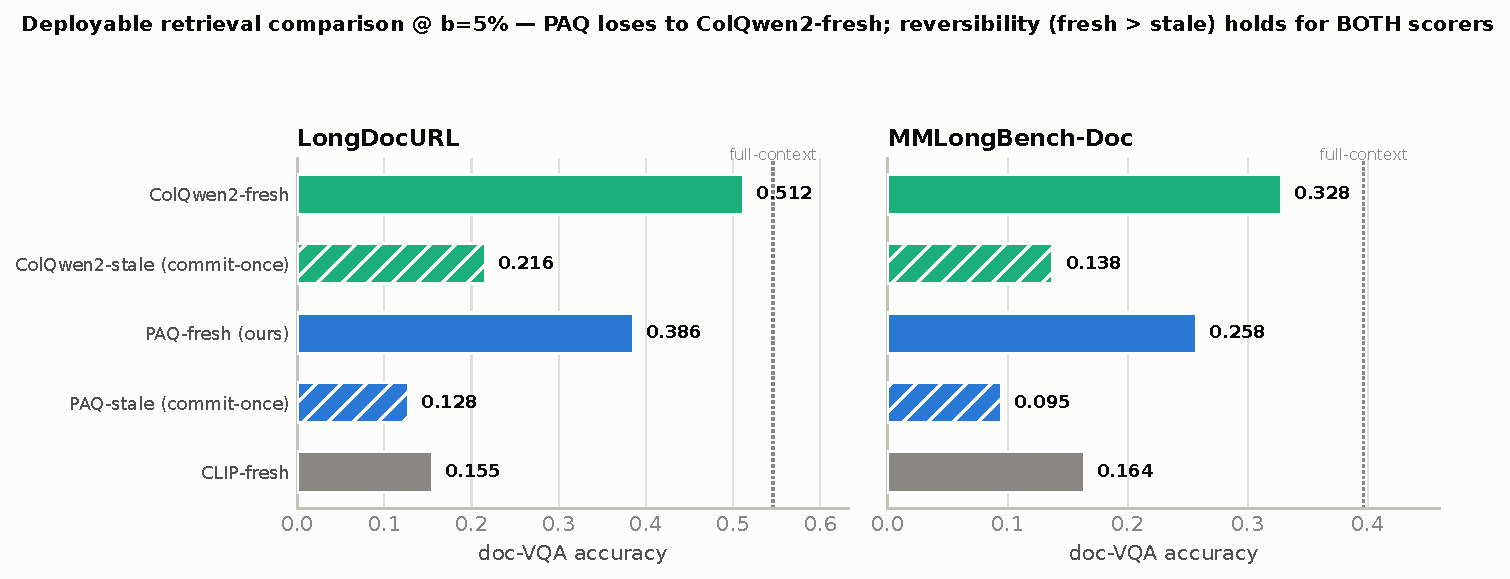
\includegraphics[width=\columnwidth]{fig_e_retrieval_reversal_light.pdf}
\caption{Two observations from the page-level system, per cell: (i) ColQwen2-fresh outperforms the page-level attention router (a loss of roughly 10 points for the router); (ii) \emph{both} scorers collapse when committed once, so reversibility is a general property of the multi-query regime rather than being scorer-specific. \paq{} here is the earlier page-level router of this appendix, not \paqc{}; the below-page \paqc{} comparison at matched budget is in Table~\ref{tab:paqkv}.}
\label{fig:retrieval}
\end{figure}

\paragraph{\paqt{}: expert-head recall and the parity accuracy evaluation.} Scoring with a single expert (layer, head) chosen by held-out-document cross-validation (CAPS's technique) lifts held-out gold-page recall@5\% to $0.683$ ($n{=}451$) / $0.626$ ($n{=}425$), meeting or exceeding ColQwen2's in-harness $0.664$/$0.536$; mean aggregation at higher scoring resolution moves almost nothing ($0.494/0.443 \to 0.500/0.452$), so the head, not the resolution, is the lever. All selected fold heads sit in layer 21. The pre-registered accuracy evaluation (bars frozen before the run; same reader, render policy, and scorer as the cached baseline rows; only the selected page set differs) lands at parity: \paqt{} $0.518$/$0.357$ vs.\ ColQwen2-fresh $0.512$/$0.328$; deltas $+0.006$ $[-0.018,+0.030]$ and $+0.028$ $[+0.001,+0.055]$; pooled $+0.017$ $[-0.000,+0.035]$. This is non-inferior under the frozen $\lb > -0.03$ margin on both cells but not the pre-registered improvement criterion (all $\lb>0$), and we do not present the marginal per-cell interval as evidence of superiority. The initially better-looking complete-case verdict (pooled $+0.023$, $\lb=+0.005$) was blocked in review for informative missingness: the ${\approx}4\%$ of queries whose high-resolution scoring ran out of memory had cached baseline accuracy $0.62$, far above the cell means; a conservative reduced-resolution recovery of 31/35 missing rows (degrading only the \paqt{} arm, never the baseline) erased the pooled edge. Two caveats carry over: head selection is cross-validated \emph{benchmark-supervised} model selection (not zero-shot; the externally selected L21.H18 of the negative transfer-gate ablation later removed this caveat from the head's existence, though not from its benchmark-tuned use), and the expert-head technique is CAPS's, so the residual novelty at page level is only the amortized one-prefill-many-queries architecture.

\section{Additional Reversibility Detail}\label{app:reversibility}

% Figure sources: BASED/research/paq_verdict.json; BASED/research/paq_revcrop_verdict.json;
%                 BASED/research/paqc_mmlongdoc_audit_verdict.json

\begin{figure*}[t]
\centering
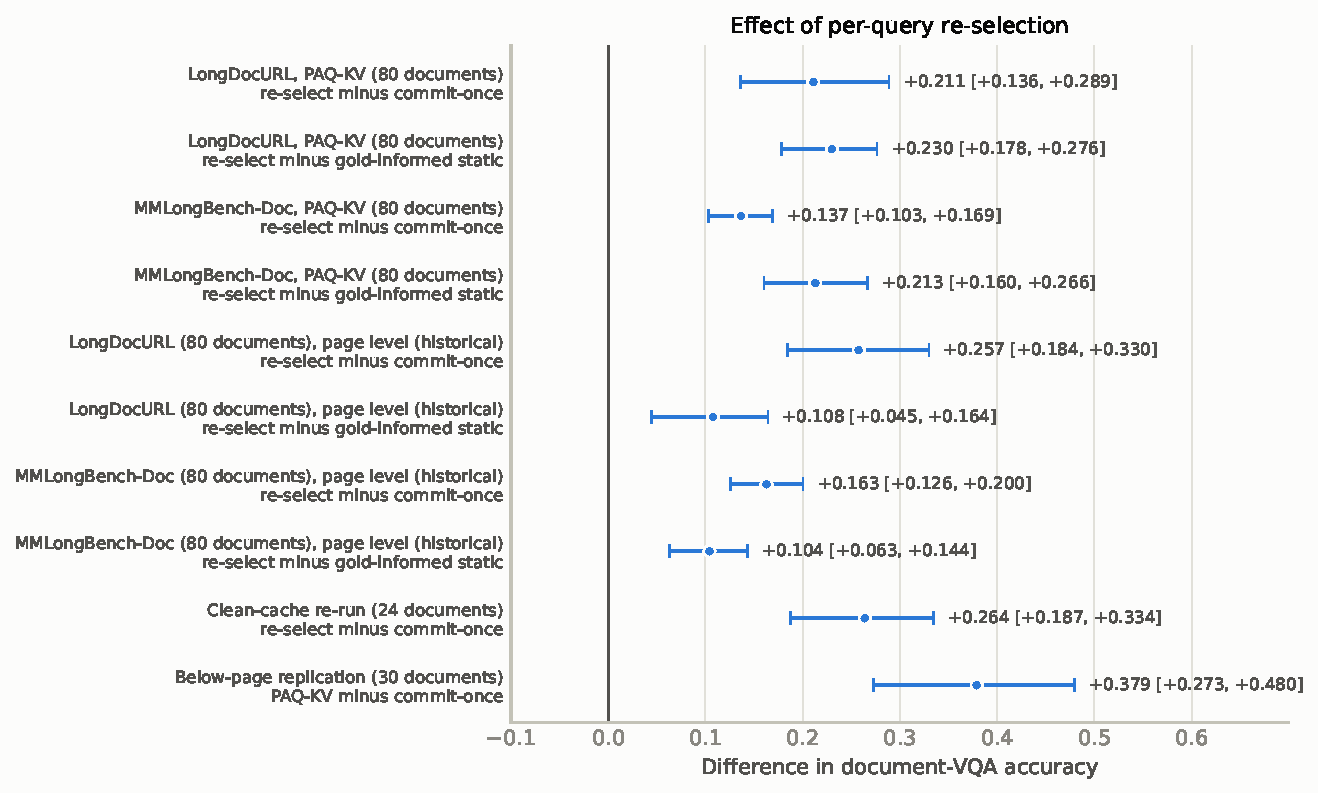
\includegraphics[width=0.92\textwidth]{fig_j_reversibility_light.pdf}
\caption{Document-clustered two-sided 95\% intervals for the confirmatory page-level contrasts, the clean-cache re-run, and the below-page \paqc{} replication. Positive differences favor per-query re-selection; every interval excludes zero.}
\label{fig:reversibility}
\end{figure*}

Figure~\ref{fig:reversibility} summarizes the confirmatory reversibility contrasts and their clean-cache and below-page replications. Additional pre-registered analyses: (i) \emph{answerable subset} (secondary, since it conditions on a model outcome): on queries where oracle-evidence scores exactly 1 ($n=407$), fresh $0.583$ vs.\ commit-once $0.182$ ($+0.395$ $[+0.324,+0.460]$) and vs.\ the static $0.382$ ($+0.204$ $[+0.135,+0.266]$); (ii) \emph{missingness}: 4 of 907 vision queries are missing due to a per-document timeout, and worst-case imputation in either direction leaves the gate verdict unchanged; (iii) \emph{budget curves}: the fresh selector dominates both static comparators at every budget in $\{2.5, 5, 10\}\%$ on both cells; at $b=10\%$ on LongDocURL it reaches $0.518$ vs.\ full-context $0.546$, so reading 10\% of pages recovers ${\approx}95\%$ of full-context accuracy on that cell (not on MMLongBench-Doc: $0.317$ vs.\ $0.397$).

\paragraph{Cache-pollution quantification.} The in-place cache bug of the main text was quantified before being fixed: on a 6-documents-per-cell diagnostic (87 query-rows), the bug inflates gold-page recall by ${\approx}+0.05$ for a fixed scoring head and shifts selections (mean top-$B$ Jaccard clean vs.\ polluted $0.82$, drifting from $1.00$ at $q_0$ to $0.61$ at $q_6$), as expected for cumulative contamination. The recall gate behind the \paqt{} numbers was regenerated clean before any accuracy read (clean held-out expert recall $0.683$/$0.626$ vs.\ polluted $0.674$/$0.628$), and the clean cross-validation picks a more robust head. Absolute fresh-arm accuracy in the pre-fix confirmatory run carries ${\approx}0.04$ inflation (clean $-$ polluted $-0.041$ $[-0.077,-0.003]$ on the 24-document check); the isolation contrasts cancel the bug and stand.

\section{Reproducibility and Protocol Notes}\label{app:repro}

\paragraph{Pre-registration discipline.} Every gate in this study was frozen (bars, comparators, budgets, imputation policy) before its run: the two-comparator isolation gate; the \paqt{} accuracy-evaluation bars (non-inferiority/improvement/inferior margins, per-cell power floors, adversarial missingness imputation); the per-head-mixture transfer gate; and the \paqc{} decode-identity kill criterion, screen gates, per-cell improvement bars, and sharp-scorer (V1) gate. Two early positives did not survive adversarial review and were retracted before this draft: a first isolation gate against the eviction family (invalidated by a weak-static artifact and replaced by the two-comparator gate), and an early ``outperforms the gold-page oracle'' claim (corrected to ``matches'' at power). The commitment-pressure mechanism hypothesis failed its formal test and is reported as exploratory.

\paragraph{Instrumentation.} All significance statements use one instrument: the document-cluster paired bootstrap (10{,}000 draws, seed 0, percentile intervals; equal-cell pooling), unit-tested alongside the gate and pairing logic. Evaluation pins are sha-256 checksummed and byte-verified before use; the screen pin is a strict prefix of the confirmatory pin, and independent-extension analyses use the 50 new documents per cell only. Figures are generated from the verdict artifacts by a single script; nothing is hand-entered. Per-query, per-arm rows, frozen-bar metadata, verdict files, and the adversarial review trail are retained and will be released with the code.

\paragraph{Sealed-test protocol.} The 80-document confirmatory pin has been reused across this study and is therefore development-only. The fresh sealed set (zero overlap with the pin; 45 MMLongBench-Doc documents / 244 queries, plus 73 LongDocURL documents left unevaluated as out of scope) was evaluated \emph{exactly once} under a guarded, frozen harness: the confirmatory bar (complete-case document-clustered $\lb>0$, with an adversarial worst-case-imputation fallback binding only under any missingness), the corrected-loader comparator, the 5\% budget, the seed, and sha-256 hashes of all eight code components plus the sealed pin were frozen before the run; the harness refuses the sealed pin absent an explicit authorization flag and a typed confirmation, aborts on any component-hash mismatch, and runs a blind non-scoring preflight that can abort without consuming the test. The single run produced the strongest claim in this paper: \paqc{}@5\% $0.396$ vs.\ ColQwen2-fresh $0.320$, $+0.076$, document-clustered $\lb=+0.029$ ($244/244$ complete, zero skips, robust to adversarial imputation; \S\ref{sec:results-mmlo}). The verdict, per-query rows, and a provenance manifest (pin and component hashes, resolved model revisions) are retained and released with the code.

\section{Additional Method and Gate Tables}\label{app:method-materials}

\begin{algorithm}[t]
\caption{\paqc{}: per-query reversible below-page KV-block selection with a 4D restricted-attention mask}
\label{alg:paqc}
\begin{algorithmic}[1]
\REQUIRE document pages rendered as in the full-context arm ($\le$64K tokens); queries $q_1,\ldots,q_k$; nominal budget $b=5\%$; frozen VLM
\STATE prefill the document once; retain the full KV cache $C$ (context length $n_{\mathrm{ctx}}$); record page-aligned 64-token block spans $B_1,\ldots,B_m$ and the always-keep scaffold set $A$
\FOR{each query $q_j$}
\STATE forward the tokenized question over $C$; capture question$\to$context attention via per-layer hooks; \textbf{crop} $C$ back to $n_{\mathrm{ctx}}$
\STATE $\mathrm{score}(B_i) \gets$ aggregated question-row attention mass on block $B_i$'s positions
\STATE $S_j \gets$ top blocks by score at the nominal budget $b \cdot n_{\mathrm{ctx}}$
\STATE build the 4D additive mask $M_j$: decode rows may attend to $A \cup S_j \cup q_j \cup{}$generated tokens; all other context positions get $-\infty$
\STATE decode the answer from $C$ under $M_j$; no gathering, so K/V positions and M-RoPE indices are unchanged
\STATE discard $M_j$; $C$ is intact for $q_{j+1}$
\ENDFOR
\end{algorithmic}
\end{algorithm}

\begin{table}[t]
\centering\small
\setlength{\tabcolsep}{4pt}% permitted narrowing (AAAI kit)
\begin{tabular}{lcc}
\toprule
 & LongDocURL & MMLongBench \\
\midrule
Documents & 80 & 80 \\
Complete queries at gate & 463 & 440 \\
Gold-bearing queries / doc & 5.79 & 5.50 \\
Median (mean) union pages & 44 (45.0) & 28 (36.5) \\
\bottomrule
\end{tabular}
\caption{The confirmatory evaluation pin. ``Complete queries'' are rows where every gated arm scored; 4 of 907 vision queries are missing due to a per-document timeout, and worst-case imputation leaves every gate verdict unchanged.}
\label{tab:pins}
\end{table}

\begin{table*}[t]
\centering\small
\begin{tabular}{lccc}
\toprule
Contrast at $b{=}5\%$ & LongDocURL & MMLongBench-Doc & pooled (equal-cell) \\
\midrule
fresh $-$ same-scorer commit-once & $+0.257$ $[+0.184,+0.330]$ & $+0.163$ $[+0.126,+0.200]$ & $+0.210$ $[+0.168,+0.250]$ \\
fresh $-$ gold-informed static & $+0.108$ $[+0.045,+0.164]$ & $+0.104$ $[+0.063,+0.144]$ & $+0.106$ $[+0.067,+0.141]$ \\
\midrule
Verdict & \multicolumn{3}{c}{\textsc{reversibility isolated} (all $\lb > 0$, both cells and pooled)} \\
\bottomrule
\end{tabular}
\caption{Confirmatory isolation at $b{=}5\%$ on 903 complete queries (accuracy; document-cluster paired bootstrap; rows report $\Delta\,[\lb,\mathrm{UB}_{95}]$). The two-comparator gate was frozen before the run.}
\label{tab:isolation}
\end{table*}

\section{Screen-Only Budget Sweep}\label{app:budget-sweep}
The improvement is not a 5\%-only artifact: \paqc{} at $2.5\%$, $5\%$, and $10\%$ all exceed ColQwen2@5\% ($+0.103$, $+0.077$, $+0.104$; the $2.5$/$10\%$ points are on the 157-query screen subset and the $5\%$ point on the full 440). Although \paqc{}'s own budget curve is mildly non-monotone here, every budget exceeds the retriever. A full-pin ColQwen2 re-read at $2.5$/$10\%$ is future work.

\section{Additional Limitations Detail}\label{app:limitations-detail}
\paragraph{LongDocURL conversion-bound decomposition.} A re-analysis of the executed rows suggests the shortfall there lies largely past selection: of the 463 rows, ${\approx}39\%$ fail under both \paqc{} and the gold-page oracle (zero even when handed the native-resolution gold pages), only ${\approx}10\%$ are oracle-right/\paqc{}-wrong (the selection-capturable pool), and $2.2\%$ are \paqc{}-right/oracle-wrong, so the oracle is not a strict ceiling; that no selection method can rescue these queries is an observation about this dataset, not a general rule. Native resolution already saturates the prefill on 79/80 documents, and large documents are a flat, low-leverage half. Among pure-selection levers, only a marginal oracle-chooser union passes ($\lb=+0.003$; not deployable); only a \paqc{}${\cup}$ColQwen2 hybrid passes comfortably ($\lb=+0.061$), and we exclude it as not a standalone method. We therefore offer the dispersed-vs-conversion-bound split as a hypothesis from two datasets.

\paragraph{Base-model ceiling counts.} A large fraction of queries receive no credit even given exactly the annotated gold pages: the oracle-evidence arm scores $0$ on $317/903=35.1\%$ of confirmatory queries and a full $1$ on only $45.1\%$. Pairing controls for shared query difficulty; the oracle is not a strict ceiling (a selected page set can score above the annotated gold set on individual queries). The query-blind eviction arms are disclosed proxies we claim nothing against.

\paragraph{Remaining protocol caveats.} The commit-once aggregate uses the first $M{=}\min(3,k)$ queries in frozen arrival order (order-permutation and $M$-sensitivity checks remain to be run; the order-free static partially covers this), and the page-level confirmatory run predates the cache fix (\S\ref{sec:integrity}); its isolation \emph{contrasts} were verified robust, but its absolute fresh-arm levels carry ${\approx}0.04$ inflation on the 24-document check.

\end{document}
